\documentclass[a4paper,11pt]{article}
\input{/home/tof/Documents/Cozy/latex-include/preambule_lua.tex}
\newcommand{\showprof}{show them}  % comment this line if you don't want to see todo environment
\fancyhead[L]{Exercices - fonctions}
\newdate{madate}{10}{09}{2020}
%\fancyhead[R]{\displaydate{madate}} %\today
%\fancyhead[R]{Seconde - SNT}
\fancyhead[R]{Première - NSI}
%\fancyhead[R]{Terminale - NSI}
\fancyfoot[L]{~\\Christophe Viroulaud}
\AtEndDocument{\label{lastpage}}
\fancyfoot[C]{\textbf{Page \thepage/\pageref{lastpage}}}
\fancyfoot[R]{\includegraphics[width=2cm,align=t]{/home/tof/Documents/Cozy/latex-include/cc.png}}
%DODO exo calcul variance, espérance (http://www.jybaudot.fr/Probas/espvariance.html)
%DODO exo en rapport avec maths: exo-maths-info.ipynb dans TOSEE/divers + méthode de monte-carlo (TP?)
\begin{document}
\begin{Form}
\begin{exo}
Écrire la fonction \textbf{est\_pair(x)} qui renvoie \emph{True} si l'entier \emph{x} est pair, \emph{False} sinon.
\end{exo}
\begin{exo}
Écrire la fonction \textbf{valeur\_absolue(x)} qui renvoie la valeur absolue de l'entier \emph{x}.
\end{exo}
\begin{exo}
Écrire la fonction \textbf{surface(r)} qui renvoie l'aire d'un cercle de rayon \emph{r}.
\end{exo}
\begin{exo}
Écrire la fonction \textbf{est\_majeur(age)} qui renvoie \emph{True} si la personne d'âge \emph{age} est majeure.
\end{exo}
\begin{exo}
Écrire la fonction \textbf{puissance(x, n)} qui renvoie \emph{x} à la puissance \emph{n}. On utilisera une boucle pour effectuer le calcul.
\end{exo}
\begin{exo}
Écrire la fonction \textbf{pythagore(a, b, c)} qui renvoie \emph{True} si le triangle formé par les côtés \emph{a, b, c} est rectangle. On supposera que les mesures sont des entiers donnés dans l'ordre croissant.
\end{exo}
\begin{exo}
Années bissextiles
\begin{enumerate}
\item Écrire la fonction \textbf{bissextile(annee)} qui renvoie \emph{True} si l'année \emph{annee} est bissextile. On rappelle qu'une année bissextile est une année multiple de 4 mais pas de 100 ou bien si elle est multiple de 400.
\item Écrire la fonction \textbf{nb\_jours(annee)} qui renvoie le nombre de jours dans l'année \emph{annee}. Cette fonction utilisera la fonction \emph{bissextile}.
\item Écrire la fonction \textbf{nb\_jours\_mois(annee, mois)} qui renvoie le nombre de jour du mois en fonction de l'année.
\end{enumerate}
\end{exo}
\begin{exo}
Écrire la fonction \textbf{nombres\_pairs(x)} qui renvoie la \emph{liste} de tous les nombres pairs inférieurs à l'entier \emph{x}.
\end{exo}
\begin{exo}
Écrire la fonction \textbf{diviseur(a)} qui renvoie la \emph{liste} de tous les diviseurs de l'entier \emph{a}.
\end{exo}
\begin{exo}
Écrire la fonction \textbf{est\_premier(x)} qui renvoie \emph{True} si l'entier \emph{x} est un nombre premier.
\end{exo}
\begin{exo}
\begin{enumerate}
\item Écrire la fonction \textbf{aleatoire\_100(n)} qui renvoie une liste de \emph{n} éléments compris entre 0 et 100.
\item Écrire la fonction \textbf{position(tableau, element)} qui renvoie l'indice de \emph{element} dans un \emph{tableau} de 50 entiers aléatoires compris entre 0 et 100. La fonction renverra -1 si \emph{element} n'est pas présent.
\end{enumerate}
\end{exo}
\begin{exo}
Écrire la fonction \textbf{nb\_voyelles(mot)} qui renvoie le nombre de voyelles dans \emph{mot}.
\end{exo}
\begin{exo}
Turtle
\begin{enumerate}
\item Écrire une fonction \textbf{triangle(c)} qui trace un triangle de côté \emph{c}.
\item Écrire le programme qui affiche la figure \ref{sapin}.
\begin{center}
\centering
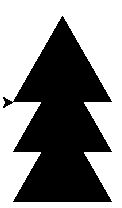
\includegraphics[width=2cm]{ressources/sapin.png}
\captionof{figure}{Sapin}
\label{sapin}
\end{center}
\end{enumerate}
\end{exo}
\end{Form}
\end{document}
